\documentclass[12pt,letterpaper]{article}

% ---------------------------------------------------------------- packages
\usepackage[T1]{fontenc}
\usepackage[utf8]{inputenc}
\usepackage{newtxtext,newtxmath}          % Times-style text and maths
\usepackage[margin=1in]{geometry}         % 6.5in text width = figure width
\usepackage{microtype}
\usepackage{graphicx}
\usepackage{booktabs}
\usepackage{tabularx}
\usepackage{array}
\usepackage[font=small,labelfont=bf,labelsep=period,skip=5pt]{caption}
\usepackage[dvipsnames]{xcolor}
\usepackage{enumitem}
\usepackage{titlesec}
\usepackage{fancyhdr}
\usepackage{placeins}                     % \FloatBarrier keeps figures in their section
\usepackage{xurl}                         % allow line breaks anywhere in URLs
\usepackage[hidelinks]{hyperref}
\usepackage[capitalise,nameinlink]{cleveref}

\graphicspath{{../figures/}}
\definecolor{ink2}{HTML}{52514E}
\definecolor{rule}{HTML}{C3C2B7}

% Compact but readable section headings.
\titleformat{\section}{\large\bfseries}{\thesection}{0.6em}{}
\titleformat{\subsection}{\normalsize\bfseries}{\thesubsection}{0.6em}{}
\titlespacing*{\section}{0pt}{10pt plus 2pt minus 2pt}{4pt}
\titlespacing*{\subsection}{0pt}{7pt plus 2pt minus 1pt}{3pt}
\setlength{\parskip}{3pt}
\setlength{\parindent}{0pt}
\setlist{itemsep=1pt,topsep=2pt,parsep=0pt,leftmargin=1.4em}
\setlength{\textfloatsep}{10pt plus 2pt minus 2pt}
\setlength{\floatsep}{8pt plus 2pt minus 2pt}
\renewcommand{\topfraction}{0.9}
\renewcommand{\textfraction}{0.08}
\renewcommand{\floatpagefraction}{0.85}

\pagestyle{fancy}
\fancyhf{}
\renewcommand{\headrulewidth}{0pt}
\fancyfoot[C]{\small\thepage}
\fancyhead[R]{\small\color{ink2}Less Fish, More Money}

\newcommand{\fig}[1]{\cref{#1}}

% ================================================================= document
\begin{document}

% ---------------------------------------------------------------- title page
\begin{titlepage}
\thispagestyle{empty}
\centering
\vspace*{1.2in}
{\small\scshape COMP 6934 \quad Data Visualization \quad Fall 2026\par}
\vspace{0.35in}
{\color{rule}\rule{\linewidth}{0.6pt}\par}
\vspace{0.25in}
{\LARGE\bfseries Less Fish, More Money\par}
\vspace{0.12in}
{\Large Three Decades of Change in Canada's\\[2pt] Commercial Sea Fisheries, 1990--2024\par}
\vspace{0.25in}
{\color{rule}\rule{\linewidth}{0.6pt}\par}
\vspace{0.4in}
{\large Final Project Report\par}
\vspace{0.1in}
{\large Group 16\par}
\vspace{0.45in}
\begin{tabular}{@{}l@{\hspace{3em}}l@{}}
\toprule
\textbf{Group member} & \textbf{Student ID} \\
\midrule
Utsav Karki          & 202683489 \\
Lata Airee           & 202680103 \\
Abishek Paudel       & 202684964 \\
\bottomrule
\end{tabular}
\vfill
{\small Memorial University of Newfoundland\\
Department of Computer Science\\[4pt]
\today\par}
\end{titlepage}

\setcounter{page}{1}

% ---------------------------------------------------------------- 1
\section{Introduction}

Few industries are as bound up with the identity of Atlantic Canada as commercial fishing,
and few have changed as dramatically in living memory. In July 1992 the federal government
closed the northern cod fishery off Newfoundland and Labrador after the stock collapsed,
ending a fishery that had operated for almost five centuries and putting tens of thousands of
people out of work~\cite{hutchings1994,rose2015}. The moratorium is usually told as a story of loss.
The data tell a more complicated story: the industry that emerged afterwards is smaller in
tonnage but larger in value, and it is built on a very different set of species.

\textbf{Dataset.} We use the \emph{Commercial Seafisheries Landings, 1990--2024} table published by
Fisheries and Oceans Canada (DFO), drawn from its Zonal Interchange File database~\cite{dfo2025}.
Each of its 10{,}640 records gives, for one year, one geography and one species, the landed
quantity (kilograms, live weight) and the landed value (Canadian dollars paid to harvesters at
the dock). It covers 35 years (1990--2024), the five Atlantic provinces, British Columbia, and
Atlantic and national totals, and 33 species or species categories organised into four groups:
groundfish, pelagics, shellfish and ``other'' (mainly marine plants). DFO suppresses 695
provincial species cells (marked ``x'') for confidentiality; all group and national totals are
complete. To compare dollars across three decades we deflate all values to constant 2024 dollars
using the Statistics Canada all-items Consumer Price Index~\cite{statcan_cpi}.

\textbf{Why it matters.} Landings are the first link in a seafood export sector worth several
billion dollars a year, and they are the main source of income in hundreds of coastal
communities. The dataset spans the whole post-collapse period, so it lets us see not just
\emph{that} the fishery changed, but how the change was distributed across species, prices and provinces,
and what kind of fishery Canada now depends on.

% ---------------------------------------------------------------- 2
\section{Research Questions}

\begin{enumerate}[label=\textbf{Q\arabic*.}, leftmargin=2.4em]
  \item \textbf{Growth or decline?} Has Canada's sea fishery grown or shrunk since 1990, and does the
        answer depend on whether it is measured in tonnes or in inflation-adjusted dollars?
  \item \textbf{What replaced groundfish?} Which species groups and species filled the gap left by
        the collapse of cod and other groundfish?
  \item \textbf{Quantity or price?} Is the growth in value driven by catching \emph{more}, or by each
        kilogram being worth more?
  \item \textbf{Who, and at what risk?} How were these shifts distributed across provinces, and
        what new risks does the resulting structure create?
\end{enumerate}

% ---------------------------------------------------------------- 3
\section{Data Preparation and Design Choices}

The DFO file is a report-style CSV, so we (i)~removed six trailing footnote lines, (ii)~converted
text numbers with thousands separators to numeric values, and (iii)~coded the confidential ``x''
cells as missing rather than zero so that they could never silently deflate a total. We then
verified that the table is internally consistent: species-group subtotals sum to the grand
total, the five Atlantic provinces sum to the Atlantic total, and Atlantic plus British Columbia
equals Canada, each to within $10^{-5}$ relative error. Analyses by province therefore use DFO's
complete group subtotals, never sums of partially suppressed species rows. Derived measures are
\emph{real value} (2024 CAD), \emph{real price per kilogram} (real value\,/\,quantity) and
\emph{year-over-year change} in real value. All processing and plotting is done in Python with
\texttt{pandas}, \texttt{seaborn}, \texttt{matplotlib} and \texttt{scipy} in a single Jupyter notebook.

Three design rules apply to every figure. First, \textbf{colour always encodes the species group}
(groundfish \textcolor[HTML]{2A78D6}{\textbf{blue}}, pelagics \textcolor[HTML]{1BAF7A}{\textbf{green}},
shellfish \textcolor[HTML]{EB6834}{\textbf{orange}}); the palette was checked with a
colour-vision-deficiency simulator, and every series is also labelled directly. Second, measures
on different scales are never drawn against two y-axes; they are indexed to a common base or
placed in separate panels. Third, each figure was drawn at its final printed width so that no
text is rescaled.

% ---------------------------------------------------------------- 4
\section{Findings}

\subsection{Q1 --- A smaller catch that is worth more}

\begin{figure}[!htb]
  \centering
  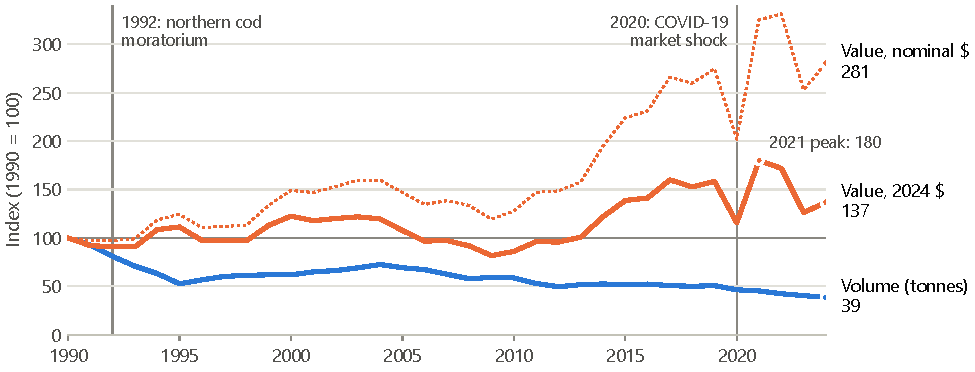
\includegraphics[width=\linewidth]{fig1_volume_vs_value}
  \caption{\textbf{Line chart: landed volume vs.\ landed value, Canada, indexed to 1990\,=\,100.}
  Volume (blue) fell to 39\% of its 1990 level, while real value (solid orange, 2024 dollars) rose
  to 137\%. Nominal value (dotted) is shown to make clear how much of the apparent growth is
  inflation. Indexing both measures to 1990 lets them share one axis. Supports Q1.}
  \label{fig:index}
\end{figure}

\Cref{fig:index} answers the first question directly, and the answer depends entirely on the unit
of measurement. By weight, the fishery has shrunk by 61\%, from 1.62~million tonnes in 1990 to
0.63~million tonnes in 2024. Most of the fall happened in the five years after the 1992
moratorium, and a fitted log-linear trend confirms a steady decline of 1.7\% per year over the
whole period ($R^2=0.71$, $p<10^{-9}$). By value, the picture is reversed. Nominal landed value
nearly tripled (\$1.43B to \$4.01B), but 58\% of that apparent gain is inflation.
In constant 2024 dollars the increase is a more modest but still clear 37\% (\$2.93B to \$4.01B;
trend $+1.3\%$ per year, $p<10^{-4}$). As a result, the average real value of a landed kilogram
rose 3.5-fold, from \$1.81 to \$6.40. The value line is also far more volatile than the volume
line: it dropped 27\% in the 2020 COVID-19 market shock, reached a record \$5.27B in 2021 and
fell back by 30\% by 2023. \Cref{sec:risk} traces that volatility to a single species.

\FloatBarrier
\subsection{Q2 --- Shellfish replaced groundfish}

\begin{figure}[!htb]
  \centering
  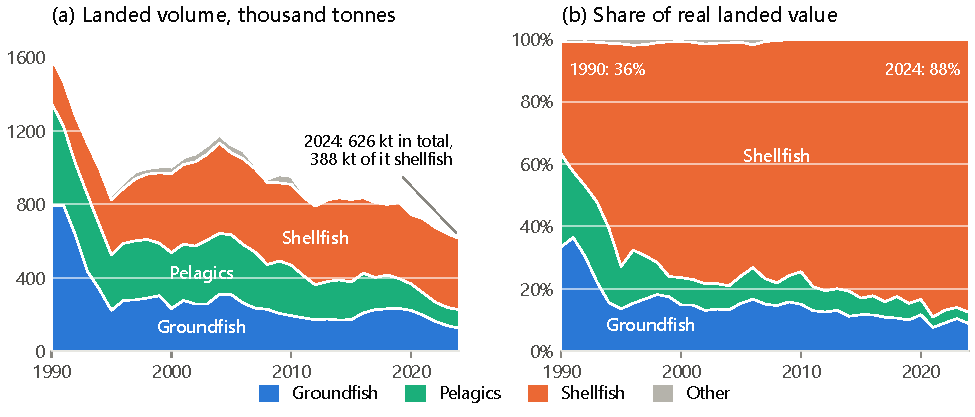
\includegraphics[width=\linewidth]{fig2_group_composition}
  \caption{\textbf{Stacked area charts by species group, Canada.} (a)~Landed volume collapsed as
  groundfish and pelagics declined, while shellfish volume held roughly steady. (b)~Shellfish's
  share of real landed value rose from 36\% (1990) to 88\% (2024). Supports Q1 and Q2.}
  \label{fig:groups}
\end{figure}

\Cref{fig:groups}a shows where the tonnes went. Groundfish landings fell from 792 to 124 thousand
tonnes (kt) and pelagics (herring, capelin, mackerel, salmon) from 559 to 101~kt. Shellfish
volume, in contrast, rose through the 1990s and has held between 380 and 490~kt since 1999. Because
shellfish are worth much more per kilogram, this change in composition dominates value
(\cref{fig:groups}b). Shellfish went from just over a third of landed value to 88\%, while
groundfish fell from 33\% to 9\% and pelagics from 30\% to 4\%.

\begin{figure}[!htb]
  \centering
  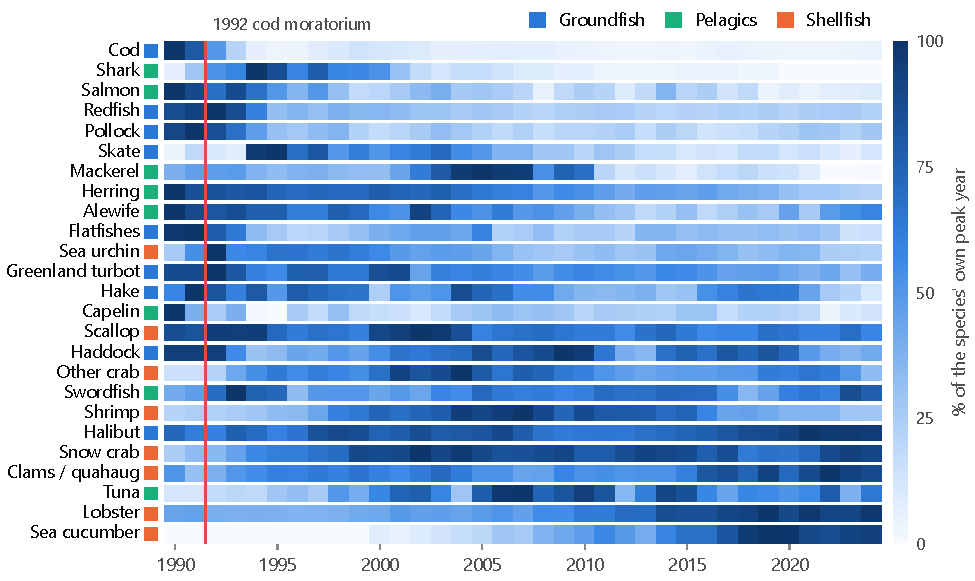
\includegraphics[width=\linewidth]{fig3_species_heatmap}
  \caption{\textbf{Heatmap: landed volume of each species as a percentage of its own 1990--2024
  peak.} Rows are ordered by the volume-weighted mean year of landings, so early-peaking
  fisheries are at the top and growing fisheries at the bottom. The coloured chip gives the species
  group. Species that never reached 1{,}000~t in any year are omitted. Supports Q2.}
  \label{fig:heatmap}
\end{figure}

The heatmap in \cref{fig:heatmap} shows that the collapse went well beyond cod. Normalising each
species to its own peak allows fisheries of very different sizes to be compared on one scale.
Thirteen of the 33 species categories, including cod, herring, capelin, salmon, redfish, pollock, flatfishes and
Greenland turbot, recorded their largest landings between 1990 and 1992 and never returned to
them. The dark cells for cod end abruptly at the moratorium line: cod landings fell from 402~kt
in 1990 to 15~kt by 1995 and were still only 18~kt in 2024, which is consistent with the slow and
incomplete recovery reported for the northern stock~\cite{rose2015}. The bottom of the chart is
where the growth happened. Snow crab, lobster, clams, halibut and sea cucumber all reached their
peaks in the last decade, and lobster and sea cucumber are still near record highs. This matches
the ecological argument that removing a top predator such as cod allowed its invertebrate prey to
flourish~\cite{frank2005}.

\begin{figure}[!htb]
  \centering
  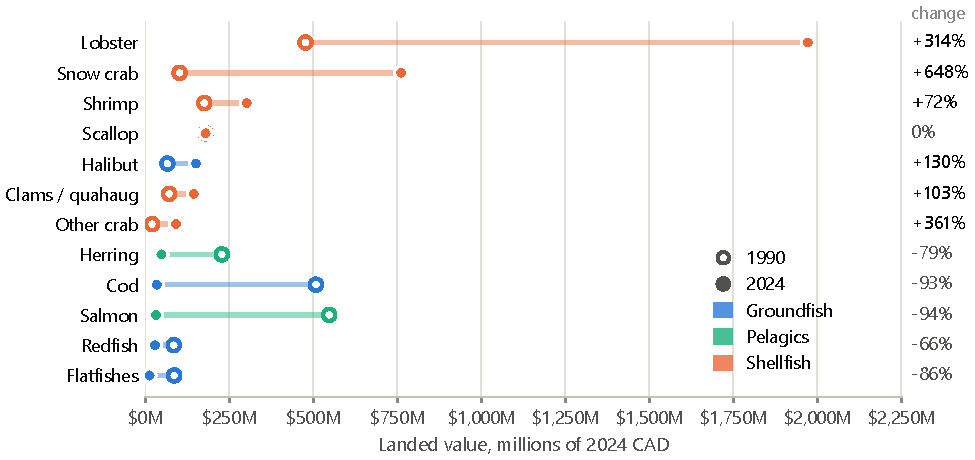
\includegraphics[width=\linewidth]{fig4_species_dumbbell}
  \caption{\textbf{Dumbbell chart: real landed value by species, 1990 (hollow) vs.\ 2024 (filled),
  millions of 2024 CAD.} Species worth at least \$60M in either year are shown, sorted by 2024
  value. The right-hand column gives the percentage change. Supports Q2.}
  \label{fig:dumbbell}
\end{figure}

\Cref{fig:dumbbell} converts this shift into dollars and names the winners and losers. Lobster's
real value quadrupled (\$477M to \$1{,}972M, $+314\%$) and snow crab's grew more than seven-fold
(\$102M to \$761M, $+648\%$). Together they added \$2.15B in real value, almost twice the \$1.17B
lost by cod ($-93\%$), salmon ($-94\%$) and herring ($-79\%$) combined. The losers are
predominantly blue and green and the winners orange, so the chart also shows the group-level
shift at species level.

\FloatBarrier
\subsection{Q3 --- Growth came from price as much as from quantity}

\begin{figure}[!htb]
  \centering
  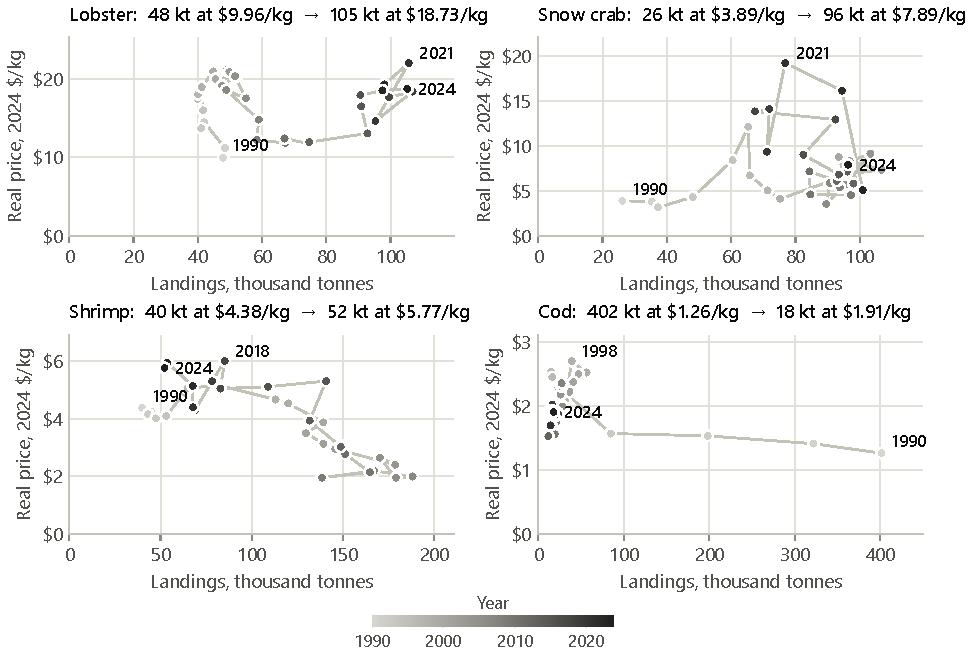
\includegraphics[width=\linewidth]{fig5_price_quantity}
  \caption{\textbf{Connected scatter plots: annual landings (x) against real price per kilogram (y)
  for four key species.} Each dot is one year, and dots darken from 1990 to 2024. Lobster moved
  up and to the right (more volume \emph{and} higher prices). Snow crab's price swung widely at
  roughly constant volume. Shrimp grew and then shrank. Cod lost 96\% of its volume, and higher
  prices could not make up for it. Supports Q3.}
  \label{fig:scatter}
\end{figure}

Value is quantity times price, and \cref{fig:scatter} separates the two for the four most
important species. Each follows a different path. \textbf{Lobster} is the only one that grew on
both axes. Landings more than doubled (48 to 105~kt) while the real price almost doubled
(\$9.96 to \$18.73/kg), peaking at \$22/kg in 2021. \textbf{Snow crab} volume rose until
the early 2000s and has since stayed between 67 and 107~kt, yet its real price since 2002 has ranged from
\$3.54 to \$19.18/kg. Almost all of its recent value changes are therefore price changes, which
move the path up and down rather than left and right. \textbf{Shrimp} traces a loop: volume
expanded to 188~kt in 2007 at falling prices, then contracted to 52~kt. \textbf{Cod} lies almost
entirely along the x-axis. Its real price rose by half, but that is negligible next to a 96\%
loss of volume. Overall, value growth since 1990 has come from a move towards species that were
expensive to begin with, and from large price increases for those species, not from catching
more.

\FloatBarrier
\subsection{Q4 --- Every province converged on shellfish, but not equally}

\begin{figure}[!htb]
  \centering
  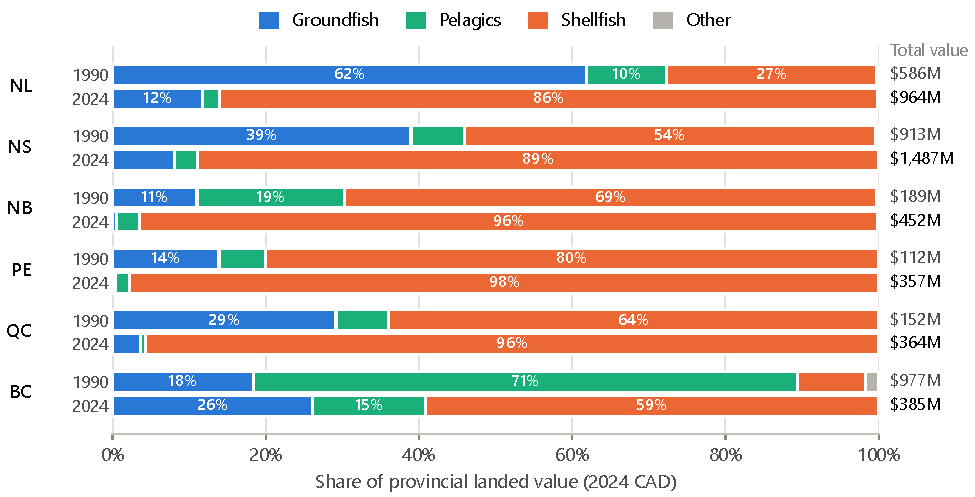
\includegraphics[width=\linewidth]{fig6_provinces}
  \caption{\textbf{100\% stacked bar chart: share of each province's real landed value by species
  group, 1990 vs.\ 2024.} Total real value (2024 CAD) is shown on the right of each bar. Segments
  below 9\% are left unlabelled. Supports Q4.}
  \label{fig:prov}
\end{figure}

\Cref{fig:prov} shows the same shift in every Atlantic province, although each started from a
different point. \textbf{Newfoundland and Labrador} changed the most: groundfish made up 62\% of its
landed value in 1990 and only 12\% in 2024, while shellfish rose from 27\% to 86\%. Even so, its
total real value grew from \$586M to \$964M. Nova Scotia (\$913M to \$1{,}487M) is now the largest
fishing province by value. New Brunswick, Prince Edward Island and Quebec each more than doubled
in real terms and now depend on shellfish for 96--98\% of their value. \textbf{British Columbia} is
the exception. Its fishery was dominated by salmon (pelagics, 71\%) in 1990, and it is the only
province whose real value fell, by 61\% (\$977M to \$385M). A shift towards shellfish there
(9\% to 59\%) was not enough to offset the loss of salmon.

\FloatBarrier
\subsection{Q4 (continued) --- Concentration and volatility}\label{sec:risk}

\begin{figure}[!htb]
  \centering
  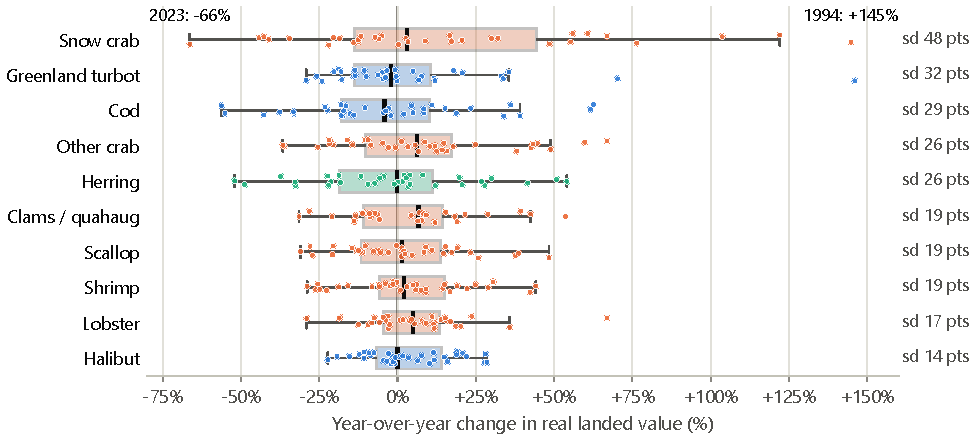
\includegraphics[width=\linewidth]{fig7_volatility}
  \caption{\textbf{Box plot with overlaid points: year-over-year change in real landed value,
  1991--2024, for the ten most valuable species of 2024.} Boxes show the interquartile range and
  the median (black bar). Each dot is one year. Rows are sorted by standard deviation (right).
  Supports Q4.}
  \label{fig:vol}
\end{figure}

The new fishery rests on a narrow base. Lobster and snow crab accounted for 20\% of national
landed value in 1990 and 68\% in 2024. Over the same period the Herfindahl concentration index
across species rose from 1{,}105 to 2{,}896, a level that competition authorities would describe
as highly concentrated. \Cref{fig:vol} shows that the two pillars behave very differently.
Lobster is one of the \emph{most stable} species: its year-to-year changes cluster tightly around a
median of $+5\%$ (standard deviation 17 points). Snow crab is by far the most volatile, with a
spread of 48 points, a $+145\%$ jump in 1994 and a $-66\%$ fall in 2023. Decomposing the variance of
the national year-to-year change in value shows that snow crab alone accounts for 49\% of it and
lobster for 36\%. Both the record in 2021 and the drop in 2023 in \cref{fig:index} are therefore
largely snow crab price cycles.

% ---------------------------------------------------------------- 5
\FloatBarrier
\section{Conclusions}

\begin{table}[h]
\centering
\small
\renewcommand{\arraystretch}{1.18}
\begin{tabularx}{\linewidth}{@{}>{\bfseries}l X l@{}}
\toprule
 & \textbf{Answer} & \textbf{Evidence} \\
\midrule
Q1 & Volume $-61\%$, real value $+37\%$; value per kg $\times3.5$. The fishery is smaller but worth more. & \fig{fig:index}, \fig{fig:groups} \\
Q2 & Shellfish (lobster, snow crab) replaced groundfish and pelagics; 13 species categories peaked in 1990--92, not only cod. & \fig{fig:groups}--\fig{fig:dumbbell} \\
Q3 & Lobster grew in both volume and price; snow crab's gains were mostly price; cod's volume loss was too large for prices to offset. & \fig{fig:scatter} \\
Q4 & Every Atlantic province converged on shellfish (NL most); BC declined. Two species now carry 68\% of value, and snow crab drives the swings. & \fig{fig:prov}, \fig{fig:vol} \\
\bottomrule
\end{tabularx}
\end{table}

\vspace{-4pt}
Taken together, the seven visualizations show that the story of Canada's fisheries since 1990
is one of \emph{substitution}, not simple decline. The collapse of groundfish and pelagic stocks
removed 60\% of the country's landed tonnage (\cref{fig:index,fig:groups}) and affected far
more than cod (\cref{fig:heatmap}). A shellfish fishery of much higher value per kilogram took its
place, and gains in lobster and snow crab alone more than paid for the dollar losses in cod,
salmon and herring (\cref{fig:dumbbell}). That growth came from prices as much as from quantity
(\cref{fig:scatter}). It reached every Atlantic province, most of all Newfoundland and Labrador,
but not British Columbia (\cref{fig:prov}).

The same evidence carries a warning. The fishery that replaced cod depends heavily on two
species, and one of them, snow crab, is driven by volatile export prices (\cref{fig:vol}).
A fishery that once risked its future on a single groundfish stock now depends on a single
family of crustaceans. Its resilience will depend on those stocks remaining healthy and on
markets beyond Canada's control.

\textbf{Limitations.} Landed value is the price paid at the dock; it excludes processing,
aquaculture and recreational catch. CPI deflation adjusts for general inflation but not for
seafood-specific costs such as fuel. Suppressed provincial cells restrict species-level
provincial analysis, which is why \cref{fig:prov} uses group totals.

% ---------------------------------------------------------------- refs
\vspace{-2pt}
\renewcommand{\refname}{\normalsize References}
{\small
\begin{thebibliography}{9}\setlength{\itemsep}{0pt}
\bibitem{dfo2025} Fisheries and Oceans Canada (2025). \emph{Commercial Seafisheries Landings, 1990--2024}. Zonal Interchange File [database], Ottawa. \url{https://www.dfo-mpo.gc.ca/stats/commercial/sea-maritimes-eng.htm}
\bibitem{statcan_cpi} Statistics Canada (2025). \emph{Table 18-10-0005-01: Consumer Price Index, annual average, not seasonally adjusted}. \url{https://doi.org/10.25318/1810000501-eng}
\bibitem{hutchings1994} Hutchings, J.\,A., \& Myers, R.\,A. (1994). What can be learned from the collapse of a renewable resource? Atlantic cod, \emph{Gadus morhua}, of Newfoundland and Labrador. \emph{Canadian Journal of Fisheries and Aquatic Sciences}, 51(9), 2126--2146.
\bibitem{rose2015} Rose, G.\,A., \& Rowe, S. (2015). Northern cod comeback. \emph{Canadian Journal of Fisheries and Aquatic Sciences}, 72(12), 1789--1798.
\bibitem{frank2005} Frank, K.\,T., Petrie, B., Choi, J.\,S., \& Leggett, W.\,C. (2005). Trophic cascades in a formerly cod-dominated ecosystem. \emph{Science}, 308(5728), 1621--1623.
\end{thebibliography}
\par\smallskip
\textit{Acknowledgement:} AI tools were used to assist with background research.\par
}

\end{document}
